We will use a subset of the Fashion MNIST dataset (\url{https://github.com/zalandoresearch/fashion-mnist}) dataset in this part. The entire dataset contains 70,000 grayscale images in 10 categories. In this HW, we will use 10,000 examples for training, 2,000 examples for validation and 10,000 examples for testing. The datapoints in the Fashion MNIST dataset are images of individual articles of clothing at low resolution (28 by 28 pixels), as seen in Fig.~\ref{fig:fmnist}:


\begin{figure}[h]
    \begin{minipage}[b]{0.45\linewidth}
    \centering
    \includegraphics[width=0.9\textwidth]{figs/fashion_mnist.png}
    \caption{Fashion-MNIST samples\protect\footnotemark}
    \label{fig:fmnist}
    \end{minipage}
    \begin{minipage}[b]{0.45\linewidth}
        \tabcolsep 20pt
        \centering
        \begin{tabular}{ll}
            \toprule
            Label &	Class \\
            \midrule
            0 &	T-shirt/top \\
            1 &	Trouser \\
            2 &	Pullover \\
            3 &	Dress \\
            4 &	Coat \\
            5 &	Sandal \\
            6 &	Shirt \\
            7 &	Sneaker \\
            8 &	Bag \\
            9 &	Ankle boot \\
            \bottomrule
        \end{tabular}
        \caption{Fashion MNIST class name}
        \label{tab:fmnist-class}
    \end{minipage}
\end{figure}

\footnotetext{Figure from \url{https://medium.com/@ipylypenko/exploring-neural-networks-with-fashion-mnist-b0a8214b7b7b}}

Fashion MNIST is intended as a drop-in replacement for the classic MNIST dataset. MNIST is often regarded as the ``Hello, World" of machine learning algorithms for computer vision. The MNIST dataset contains images of handwritten digits (0, 1, 2, etc.), and is similar in format to the Fashion MNIST dataset. This problem uses Fashion MNIST instead of MNIST to add some variety (and fashion), and also because it's slightly more challenging than regular MNIST. Both datasets are relatively small and are often used to verify that an algorithm works as expected. They're good starting points to test and debug code, and to explore ideas.

The images from Fashion MNIST are stored as 28x28 arrays, with pixel values ranging from 0 to 255. The labels are an array of integers, ranging from 0 to 9. The labels correspond to the item of clothing the image represents, as in Fig.~\ref{tab:fmnist-class}. Each image is mapped to a single label.

\newpage
\subsubsection*{Part I - Multi-Layer Perceptron (MLP) (\blue{38pts})}

\paragraph{General instructions}
\begin{itemize}
    \item In this part you will implement neural nets. We provide the bootstrap code and you are expected to complete the functions.
    \item Do not import libraries other than those already imported in the original code. 
    \item Please follow the data type annotations. You have to make the function’s return values match the required type.
    \item Only make modifications in \{\texttt{neural\_networks.py}\}.
    \item For parts where you will be running the code, we include the expected running time on Google Colab notebook in brackets (such as [\pink{5min}]). If the running time of your code is much larger, it is likely that it has a bug. Your runtime maybe much faster though (indeed, the code ran faster on our laptops than on Colab).
\end{itemize}


\textbf{3.1 Neural nets} (\blue{24pts})
In this task, you are asked to implement neural networks! You will later use this neural network to classify Fashion MNIST images into articles of clothing (0-9). The architecture of the neural network you will implement is based on the \emph{multi-layer perceptron} (also known as {MLP}, just another term for fully connected feedforward networks we discussed in class). It is designed for a $K$-class classification problem. Let $(\x,y)$ where $x\in\R^d, y\in\{1,2,...,K\}$  be a labeled instance. A MLP predicts the label by carrying out the following computations:
\begin{align*}
    \textbf{input features}: & \x\in\R^d \\
    \textbf{linear}^{(1)}: & \vct{u}=\mat{W}^{(1)}\x+\vct{b}^{(1)} \quad , \mat{W}^{(1)}\in\R^{M\times d} \ \text{and} \ b^{(1)}\in\R^M \\
    \textbf{relu}: & \vct{h} = \max\{0, \vct{u}\}=
    \begin{bmatrix} 
        \max\{0, u_1\} \\
        \vdots \\
        \max\{0, u_M\}
    \end{bmatrix} \\
    \textbf{linear}^{(2)}: & \vct{a}=\mat{W}^{(2)}\vct{h}+\vct{b}^{(2)} \\
    \textbf{softmax}: & \vct{z} = 
    \begin{bmatrix} 
        \frac{e^{a_1}}{\sum_k e^{a_k}} \\
        \vdots \\
        \frac{e^{a_K}}{\sum_k e^{a_k}} \\
    \end{bmatrix} \\
    \textbf{predicted label}: & \hat{y}=\argmax_k z_k
\end{align*}

You might find it helpful to first go through what the following parts are asking, and then read through the \texttt{main} function to see how we will be using the functions you will write. Note that to better utilize the validation set, early-stopping is provided in the starter code. Early-stopping has a hyperparameter which we call \textit{Patience}. If the patience parameter is set to $k$ \emph{epochs}, then training will terminate if there is no improvement in the validation accuracy for $k$ epochs in a row. An epoch is just one pass through the training set.  \\

\textbf{3.1.1 Linear layer} (\blue{6pts}) 
First, you need to implement the linear layer of the MLP by implementing three python functions in \texttt{class linear\_layer}. This layer has two parameters $\verb|W|$ and $\verb|b|$.

\begin{itemize}
    \item In the function \texttt{def \_\_init\_\_(self, input\_D, output\_D)}, you need to randomly initialize the entries of $\verb|W|$ and $\verb|b|$ with mean 0 and standard deviation 0.1 using \texttt{np.random.normal}. You also need to initialize the gradients to zeroes in the same function.
    \item In \texttt{def forward(self, X)}, implement the forward pass of this layer. Note that the input $\verb|X|$ contains several examples, each of which needs to be passed through this layer. Try to use matrix operation instead of for loops to speed up your code. (As you might have realized with previous homeworks, matrix operations are much faster than for loops in Python. Please read this nice guide on \emph{vectorized} operations to learn more: \url{https://www.askpython.com/python-modules/numpy/vectorization-numpy}).
    \item In \texttt{def backward(self, X, grad)}, implement the backward pass of this layer. Here, \verb|grad| is the gradient with respect to the output of this layer, and you need to find and store the gradients with respect to $\verb|W|$ and $\verb|b|$, and also find and return the gradients with respect to the input $\verb|X|$ of this layer.
\end{itemize}

\textbf{3.1.2 ReLU} (\blue{4pts})
Next, you need to implement the ReLU activation by implementing 2 python functions in \texttt{class relu}. There are no parameters to be learned in this module. 

\begin{itemize}
    \item In \texttt{def forward(self, X)}, implement the forward pass of ReLU activation.
    \item In \texttt{def backward(self, X, grad)}, implement the backward pass of ReLU activation. Here, $\verb|X|$ is the gradient with respect to the output of this layer, and you need to return the gradient with respect to the input $\verb|X|$.
\end{itemize}

\textbf{3.1.3 Mini-batch stochastic gradient descent} (\blue {2pts}) 
Next, implement mini-batch version of stochastic gradient descent to learn the parameters of the neural network. Recall that for a general optimization problem with a parameter $w$, SGD iteratively computes
$w_t = w_{t-1} - \eta \nabla F(w)$, where $\eta$ is the step size, and $\nabla F(w)$ is the stochastic gradient (at $w_{t-1}$ \textit{w.r.t} loss function $F(\cdot)$). You need to complete \texttt{def miniBatchGradientDescent(model, \_learning\_rate)}, where we update the parameters of each layer. Note that this function is executed after the backward pass of each layer has been called and the gradients have been stored properly.\\

\textbf{3.1.4 Backpropagation} (\blue {4pts}) 
Your network is almost ready to be trained. The only function you need to implement in this part is \texttt{backward\_pass}, which calls the backward pass of each layer in the correct order and with the correct inputs.\\

\textbf{3.1.5 Gradient checker} (\blue {4pts}) 
As you probably realized as you wrote the code for the previous parts, backpropagation is a subtle algorithm and it is easy to make mistakes. In this part, you will implement gradient checking to give you confidence that you are calculating the gradients of your model correctly. The idea behind gradient checking is as follows. As mentioned in the lecture, one naive way to approximate gradient is by
\begin{align*}
    \frac{dF(w)}{dw}=\lim_{\epsilon\rightarrow 0} \frac{F(w+\epsilon)-F(w-\epsilon)}{2\epsilon}
\end{align*}
We can use this relation to check that we are computing gradients correctly using backpropagation.
For example, to check the gradient of the $(0,0)$ entry of $\mat{W}^{(1)}$, we apply a small $\epsilon=1$e$-3$ perturbation to the $(0,0)$ entry of $\mat{W}^{(1)}$. Then, we compare the approximate gradient of the objective function with respect to the $(0,0)$ entry of $\mat{W}^{(1)}$ computed by the above equation, to the value obtained by backpropagation. These two values should be close to each other if backpropagation is implemented correctly. Please implement the \texttt{gradient\_checker} function to do this.
Note that to enable this function at runtime, you should turn on the \texttt{check\_gradient} flag when you run the code later.

Apart from the gradient checker, we also provide a \texttt{magnitude\_checker} function to help you debug the code. The gradient on any mini-batch provides an unbiased estimate of the true gradient, therefore we expect the gradient on a batch size of 50 to be similar in magnitude to the gradient on a batch size of 5,000. The \texttt{magnitude\_checker} function (which is provided to you) checks that the $\ell_1$-norm of $\mat{W}^{(1)}$ is of the same magnitude on these two batch sizes.\\

\textbf{3.1.6 Screenshots and plots} (\blue {4pts}) [\pink{40sec}]
After finishing all five modules above, run the below command to get a result file \texttt{MLP\_lr0.01\_b5.json}. Take a screenshot of your output log, like in \texttt{screenshot\_run\_b5.png} (included in the zip file). (\blue {2pts}) Plot the training accuracy \textit{vs.} epochs using \texttt{plot\_train\_process.py}. (\blue {2pts}) For the magnitude check, you should expect the two numbers are of the same magnitude (however, there can be small differences).. For the four gradient checks, you should expect the number from the backpropagation to be the same as that from the approximation. For training accuracy, the curve should grow as the number of epochs increases. Some fluctuation in the middle is acceptable.
$$\colorbox{Gainsboro!60!Lavender}{\texttt{python neural\_networks.py --minibatch\_size 5 --check\_gradient --check\_magnitude}}$$

\begin{figure}[H]
\centering
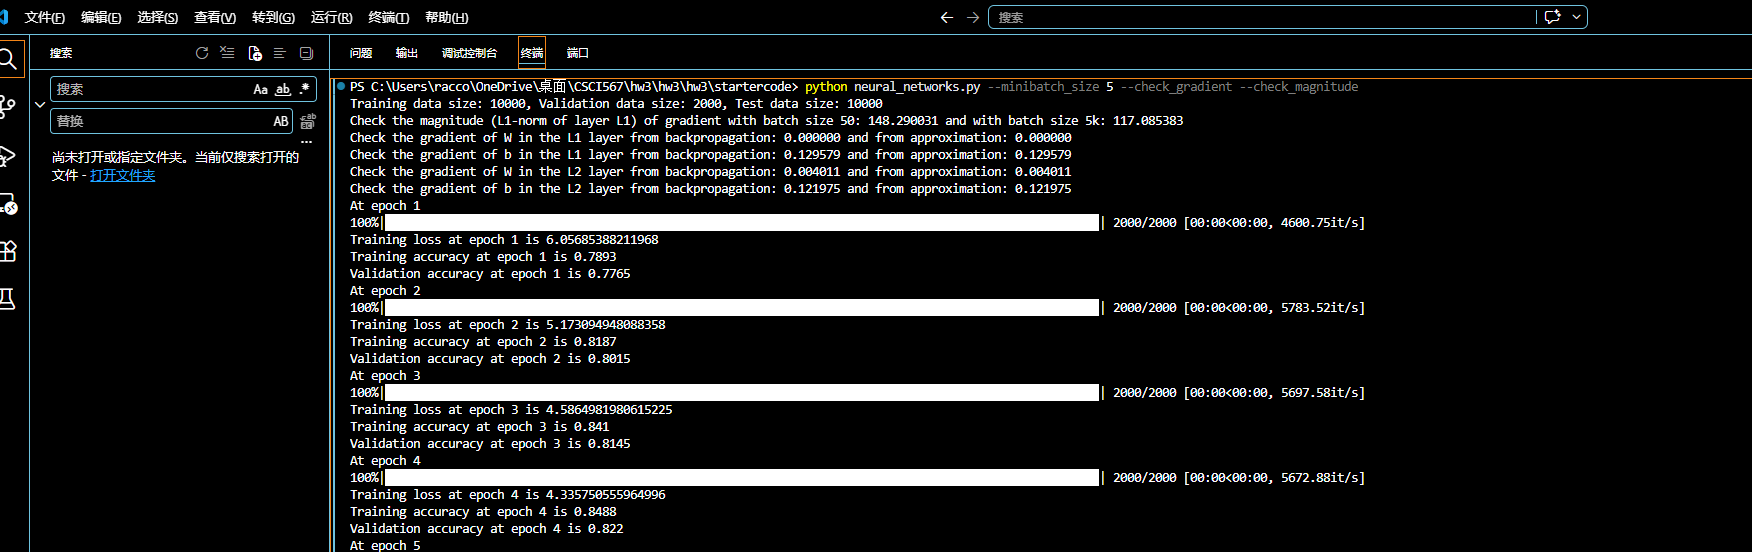
\includegraphics[width=0.6\linewidth]{screenshot.png}
\caption{Batch size = 1}
\end{figure}

\begin{figure}[H]
\centering
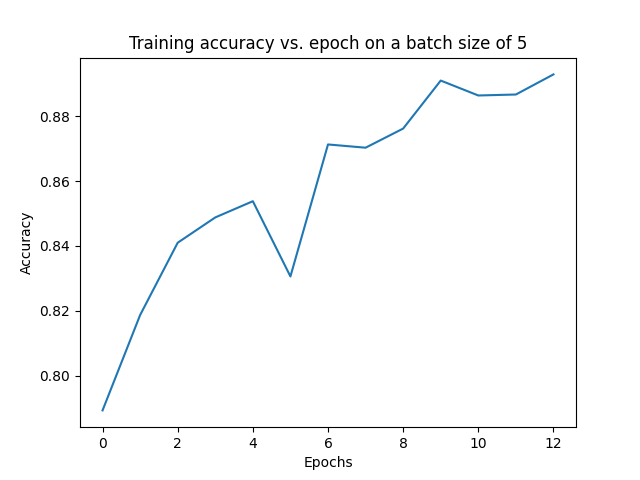
\includegraphics[width=0.6\linewidth]{train_acc_cmd.png}
\caption{Batch size = 1}
\end{figure}

\textbf{3.2 Batch size} (\blue {14pts}) [\pink{6min}]
We now explore the effect of different batch size on training. Run the command from the previous part with 5 different batch sizes: 1, 5, 50, 500, 5000. \\

\textbf{3.2.1 Accuracy and time} (\blue {4pts}) 
Plot testing accuracy and training time \textit{w.r.t.} batch size using \texttt{plot\_batch.py}.\\

\begin{figure}[H]
\centering
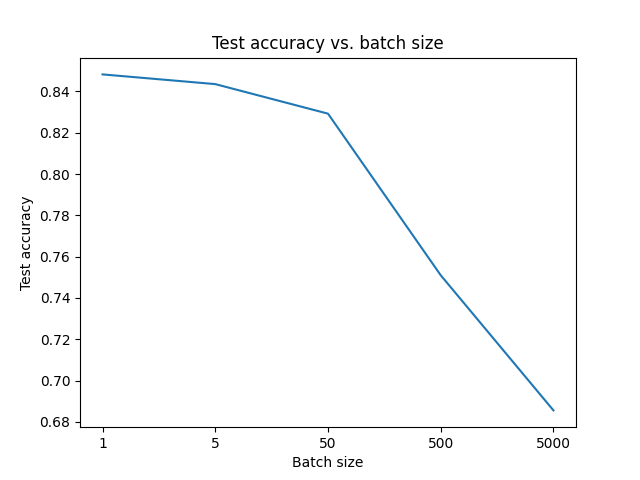
\includegraphics[width=0.5\linewidth]{test_acc.png}
\caption{Batch size = 1}
\end{figure}

\begin{figure}[H]
\centering
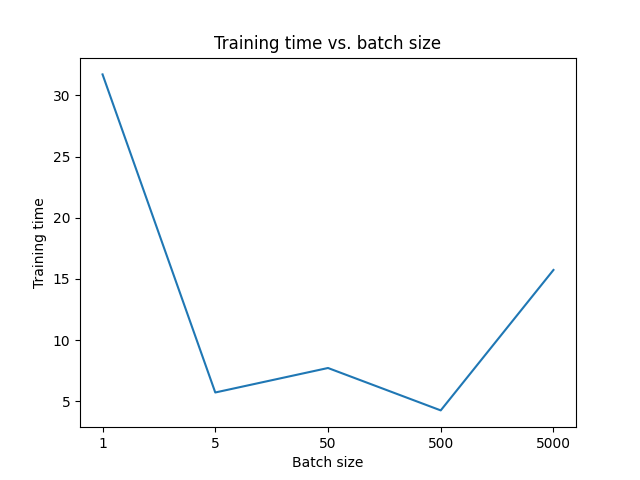
\includegraphics[width=0.5\linewidth]{train_time.png}
\caption{Batch size = 1}
\end{figure}

\textbf{3.2.2 Epochs and gradient updates} (\blue {4pts}) 
What is the number of training epochs required to get the best model for each batch size? How many gradient updates are required get the best model for each batch size? (We define a gradient update to be a single stochastic gradient descent step, where the gradient may have been computed over some mini-batch).  \\

\noindent{\fontsize{11}{12}\selectfont\textbf{Solution 3.2.2}}

The number of training epochs required to obtain the best model varies across different batch sizes. Based on our experiments:

\begin{itemize}
    \item Batch size = 1 $\rightarrow$ 16 epochs, test accuracy = 0.8482
    \item Batch size = 5 $\rightarrow$ 13 epochs, test accuracy = 0.8435
    \item Batch size = 50 $\rightarrow$ 46 epochs, test accuracy = 0.8292
    \item Batch size = 500 $\rightarrow$ 42 epochs, test accuracy = 0.7510
    \item Batch size = 5000 $\rightarrow$ 150 epochs, test accuracy = 0.6856
\end{itemize}

The number of gradient updates per epoch is given by:
\[
\text{updates per epoch} = \frac{10000}{\text{batch size}}
\]

Thus, the total number of gradient updates required to reach the best model is:

\begin{center}
\begin{tabular}{c|c|c|c}
Batch Size & Epochs & Updates/Epoch & Total Updates \\
\hline
1 & 16 & 10000 & 160000 \\
5 & 13 & 2000 & 26000 \\
50 & 46 & 200 & 9200 \\
500 & 42 & 20 & 840 \\
5000 & 150 & 2 & 300 \\
\end{tabular}
\end{center}

We observe that smaller batch sizes achieve higher test accuracy, whereas larger batch sizes lead to significantly worse performance. This suggests that smaller batches provide noisier gradient estimates that help generalize.

However, larger batch sizes require far fewer gradient updates overall, since each update processes more data. However, they often require more epochs to converge and may lead to poorer solutions.

Overall, there is a trade-off between computational efficiency (fewer updates for large batch sizes) and model performance (better accuracy for smaller batch sizes).

\bigskip

\textbf{3.2.3 Analysis} (\blue {6pts}) 
Answer the following question based on the previous plots and results:
\begin{enumerate}[(i).]
    \item Does smaller batch size guarantee faster training? Why do you think this is the case?
    \item Does larger batch size imply higher test accuracy? Why do you think this is the case?
    \item Does larger batch size imply less gradient updates to converge? Why do you think this is the case? 
\end{enumerate}

\noindent{\fontsize{11}{12}\selectfont\textbf{Solution 3.2.3}}
\subsection*{3.2.3 Analysis}

\textbf{(i) Does smaller batch size guarantee faster training?}

No, smaller batch size does not guarantee faster training. 
From our experiments, batch size = 1 achieves a high test accuracy (0.8482), but requires the longest training time (31.71 seconds). In contrast, batch size = 5 achieves comparable accuracy (0.8435) with significantly less training time (5.72 seconds). 

This is because smaller batch sizes require many more gradient updates per epoch (e.g., 10000 updates for batch size 1), which increases computational cost. Therefore, although smaller batch sizes may converge in fewer epochs, the overall training time can be longer.

\vspace{0.5em}
\textbf{(ii) Does larger batch size imply higher test accuracy?}

No, larger batch size does not imply higher test accuracy. 
In fact, our results show the opposite trend: as batch size increases, test accuracy consistently decreases (from 0.8482 at batch size 1 to 0.6856 at batch size 5000).

This happens because smaller batch sizes introduce more noise in gradient estimation, which helps the model escape sharp minima and improves generalization. In contrast, large batch sizes produce smoother gradients but tend to converge to sharper minima, leading to worse generalization performance.

\vspace{0.5em}
\textbf{(iii) Does larger batch size imply fewer gradient updates to converge?}

Yes, larger batch sizes generally require fewer gradient updates to reach convergence. 
From our experiments, the total number of updates decreases dramatically from 160000 (batch size 1) to only 300 (batch size 5000).

This is because each update with a large batch size uses more data, making the gradient estimate more stable. However, larger batch sizes often require more epochs to converge (e.g., 150 epochs for batch size 5000), and despite fewer updates, they may converge to poorer solutions.

\vspace{0.5em}
\textbf{Overall}, our experiments demonstrate a clear trade-off: smaller batch sizes lead to better generalization and higher accuracy, while larger batch sizes improve computational efficiency but may significantly degrade performance.

\newpage
\subsubsection*{Part II - Explore on Colab (\blue{12pts})}\label{colab_section}

The two-layer MLP from the previous part is our base model, and in the rest of this HW we will explore some variations on it. We will do this on a Colab notebook \texttt{fashion\_mnist.ipynb}. To run the notebook, upload the \texttt{fashion\_mnist.ipynb} to your USC Google Drive. Then, add Google Colab to your Google App by New $\rightarrow$ More $\rightarrow$ Connect more apps $\rightarrow$ Type in Google Colab and install it, as in Fig.~\ref{fig:colab-ins-1} and Fig.~\ref{fig:colab-ins-2}. After that, you can run the notebook with your browser. The notebook is based on \emph{TensorFlow}, a popular library for neural networks. TensorFlow enables us to build and train neural networks with a few simple lines of code. We recommend that you go through the TensorFlow code we provide and understand what's happening, but for the purpose of this homework you will mainly have to run the code and understand the results. 

\begin{figure}[h]
    \begin{minipage}[b]{0.5\linewidth}
    \centering
    \includegraphics[width=0.9\textwidth]{figs/colab-install-1.png}
    \caption{Colab install 1}
    \label{fig:colab-ins-1}
    \end{minipage}
    \begin{minipage}[b]{0.5\linewidth}
        \centering
        \includegraphics[width=0.9\textwidth]{figs/colab-install-2.png}
        \caption{Colab install 2}
        \label{fig:colab-ins-2}
    \end{minipage}
\end{figure}

\textbf{3.3 The effect of early-stopping} (\blue {6pts}) [\pink{3.5min}] We provided built-in early-stopping in the starter code, but did not explore the effect that it has on training. In this question, we will explore the effect of early-stopping. To do this, we evaluate the training, validation and test accuracy for each training epoch. We then plot the training, validation and test accuracy throughout the training process to see how early-stopping works.
%We provided built-in early-stopping in the starter code, but we have not explored the effect of early-stopping  yet. We evaluate the training, validation and test accuracy for each training epoch. And then, we plot these accuracies throughout the training process to see how early-stopping works. 
We train 30 epochs on a batch size of 5 without early-stopping.
\begin{enumerate}[(i).]
    \item Plot the training accuracy vs. the number of epochs. On the same graph, plot the validation and test accuracy vs. the number of epochs. Also, mark the point on the test accuracy curve where we previously early-stopped. (We provide the plotting code, you only need to run it). (\blue {2pts})
    \item What is the trend of training and test accuracy after the early-stopped point? (\blue {2pts})
    \item Based on the plot, what do you think could go wrong if the patience parameter for early-stopping is too small? (Recall that if the patience parameter is set to $k$ {epochs}, then  training will terminate if there is no improvement in the validation accuracy for $k$ epochs in a row.) (\blue {2pts})
\end{enumerate}


\textbf{3.4 SGD with momentum} (\blue {6pts}) [\pink{14min}]
We mentioned in class that adding a ``momentum" term, which encourages the model to continue along the previous gradient direction helps the network to converge. Concretely, with an initial velocity $\vv=\mathbf{0}$, we update the gradient by
\begin{align*}
    \vv & \leftarrow \alpha \vv + \nabla F(\vw) \\
    \vw & \leftarrow \vw - \eta \vv
\end{align*}
where $\eta$ is the learning rate and $\alpha$ is the factor describing how much weight we put on the previous gradients. $\alpha=0$ is equivalent to gradient update without momentum. 

We provide the \texttt{sgd\_with\_momentum} function with argument $\alpha$. In this question, we will explore how the  momentum factor $\alpha$ effects training loss and test accuracy.

\begin{enumerate}[(i).]
    \item Run the code to call the function \texttt{sgd\_with\_momentum} with $\alpha$ = 0.1, 0.3, 0.5, 0.7, 0.9. We store the training loss and test accuracy returned by the function.
    We visualize the training loss by plotting 5 curves for the 5 different values of $\alpha$ on the same graph. Each curve has the epoch on the $x$-axis and the training loss on the $y$-axis. (\blue {4pts})
    \item Based on this, what is a suitable value of $\alpha$? Therefore, how should training ideally rely on previous gradients for better convergence? (\blue {2pts})
\end{enumerate}


\newpage
\subsubsection*{Part III- Exploring Out-of-Distribution (OOD) generalization on Colab (\blue{15pts}) [\pink{15min}]}


A major research direction at present is to ensure that our ML models not only do well on test data drawn from the same distribution as training data, but that they also do well when they get data from distributions different from the original distribution. This is known as Out-of-Distribution (OOD) generalization. In the Fashion MNIST dataset, the training and test set are drawn from the same distribution. Let's explore how our models do on test data coming from a slightly different distribution.\\

\textbf{3.5 Translation and rotation (\blue{15pts})} We modify the original test datapoints, by moving up the images of the test set by 4 pixels. By doing this, we create a new translated test set. Run the code to see the original and modified images. You will notice that to a human eye, the new test set is not any more difficult than the original test set.

\begin{enumerate}[(i).]
\item But can our MLP model still do well on the new test set? What's the test accuracy on the two-layer MLP? (\blue {1pt})
\item What if we try a different model architecture? For example, in class we saw that convolutional neural networks are good at dealing with image translation. We replace the first linear layer with a convolutional layer of 64 kernels with size $7\times7$, followed by max-pooling. This can be done with just one or two lines of code in TensorFlow. Calculate the number of parameters of the CNN model and the original 2-layer MLP model (show your calculation), and verify that the CNN has fewer parameters than the MLP model. (\blue {3pts})
\item Train the 2-layer CNN on the original training data and test it on both the original and the translated test sets. What is the in-domain test accuracy and the translated test accuracy of the CNN model? Can you provide some intuition behind these numbers? (\blue {2pts}) [\pink{6min}]
\item Going one step further, we can make the CNN deeper by adding one more convolutional layer of $64\times128$ (64 input channels and 128 output channels) kernels with size $2\times2$ between the two existing layers, followed by max-pooling. Verify that the deeper 3-layer CNN model has fewer parameters than the 2-layer CNN model (show your calculation). (\blue {3pts}) 
\item What is the in-domain and the translated test accuracy of the deeper 3-layer CNN model? Provide some intuition on why it is better than the 2-layer CNN on the translated set. (\blue {3pts}) [\pink{9min}] You will notice that the deeper model takes some time to train. If we trained on GPUs instead of CPUs, training would be much faster. This is because GPUs are much more efficient at matrix computations, which is exactly what neural network training demands.
\end{enumerate}

\noindent Next, we create 3 more OOD test sets by rotation. We rotate the images in the original test set by 90, 180 and 270 degrees.

\begin{enumerate}[(vi).]
    \item Provide the test accuracy of the 2-layer MLP model, the 2-layer CNN model and the 3-layer CNN model on the three rotation test sets. Are the 2-layer CNN and the 3-layer CNN still doing well? (\blue {3pts})
\end{enumerate}


\noindent \paragraph{Deliverables for Problem 3:}
Code for 3.1 as a separate Python file \texttt{neural\_networks.py}. Screenshot for 3.1. Plots for part 3.1, 3.2, 3.3 and 3.4. Number of epochs and gradient updates for part 3.2. Analysis and explanation for parts 3.2, 3.3, 3.4. For question 3.5, submit the test accuracy on in-domain and OOD test sets of the three models, the number of parameters of the three models, and the explanations we ask for.


